%% tikz-nfold.sty
%% Copyright 2023 Jonathan Schulz
%
% This work may be distributed and/or modified under the
% conditions of the LaTeX Project Public License, either version 1.3
% of this license or (at your option) any later version.
% The latest version of this license is in
% http://www.latex-project.org/lppl.txt
% and version 1.3c or later is part of all distributions of LaTeX
% version 2008-05-04 or later.
%
% This work has the LPPL maintenance status ‘maintained’.
%
% The Current Maintainer of this work is Jonathan Schulz.
%
% This work consists of the files pgflibrarybezieroffset.code.tex, tikzlibrarynfold.code.tex,
% tikz-nfold.sty, and tikz-nfold-doc.tex.


\documentclass[12pt,a4paper]{article}

\usepackage[utf8]{inputenc}
\usepackage{tikz}
\usepackage{tkzexample}
\usetikzlibrary{calc}
\usetikzlibrary{nfold}
\usepackage{parskip}
\usepackage[margin=2.5cm]{geometry}

% recommended order: 1) hyperref 2) amsthm 3) cleveref 4) \newtheorem
\usepackage[colorlinks]{hyperref}
\usepackage{amsmath}
\usepackage{amsthm}
\usepackage[capitalize]{cleveref}

\theoremstyle{definition}
\newtheorem{definition}{Definition}[section]

\newcommand{\todo}[1]{{\color{red}\bfseries#1}}
\newcommand{\tikzdouble}{\texttt{/tikz/double}}
\newcommand{\nfold}{\texttt{nfold}}
\newcommand{\tikznfold}{\texttt{/tikz/nfold}}

\pgfkeys{/tkzexample/every tkzexample/.style={code=violet!15, graphic=orange!20, very small}}

\newcommand{\tv}{\vec{t}}
\newcommand{\uv}{\vec{u}}
\newcommand{\vv}{\vec{v}}

\begin{document}

\title{The \textsf{tikz-nfold} package}
\author{Jonathan Schulz}
\date{March 2023}

\maketitle

\begin{abstract}
  This package provides an alternative to TikZ' \verb|/tikz/double| option, avoiding some shortcomings of the original approach. It also provides an option to draw triple, quadruple, and n-fold paths.
\end{abstract}

\section*{Compatibility}
This package has been tested with \texttt{pdflatex}, \texttt{lualatex} and \texttt{xelatex}. Support for plain \TeX{} could, in principle, be implemented in the future as well.

\section{Quick start}

Add
\begin{verbatim}
\usetikzlibrary{nfold}
\end{verbatim}
to your preamble. Now you can add the style \tikznfold{} to any path that uses \tikzdouble:

\begin{tkzexample}[latex=4cm]
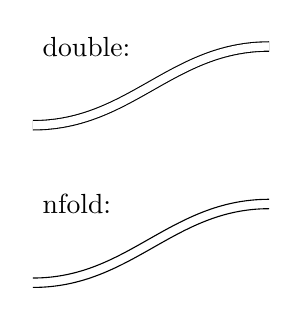
\begin{tikzpicture}
  \draw[double distance=3pt]
    (0,2) to[out=0, in=180] (3,3);
  \draw[double distance=3pt, nfold]
    (0,0) to[out=0, in=180] (3,1);
  \node[right] at (0,3) {double:};
  \node[right] at (0,1) {nfold:};
\end{tikzpicture}
\end{tkzexample}
While it appears that adding \nfold{} does not do much here, it avoids some rendering issues of \tikzdouble, hence I recommend using it in most cases (see \cref{subsec:doubleIssues} for details).

Specify a number for n-fold lines:
\begin{tkzexample}[latex=4cm]
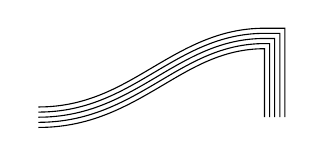
\begin{tikzpicture}
  \draw[double distance=7pt, nfold=5]
    (0,0) to[out=0, in=180] (3,1) -- (3,0);
\end{tikzpicture}
\end{tkzexample}

The arrow tips \texttt{Implies} and \texttt{Bar} are supported (the latter can also be aliased by \texttt{|}):
\begin{tkzexample}[, latex=4cm]
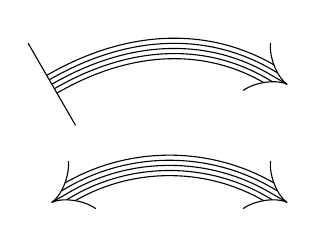
\begin{tikzpicture}
  \draw[double distance=7pt, nfold=5, arrows=Bar-Implies]
    (0,1.5) to[bend left] (3,1.5);
  \draw[double distance=7pt, nfold=5, arrows=Implies-Implies]
    (0,0) to[bend left] (3,0);
\end{tikzpicture}
\end{tkzexample}

Different line joins are supported:
\begin{tkzexample}[latex=2cm]
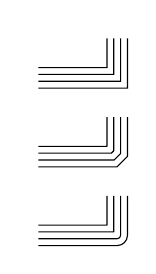
\begin{tikzpicture}[line join=bevel]
  \draw[line join=miter, double distance=7pt, nfold=4]
    (0,2) -- (1, 2) -- (1,2.5);
  \draw[double distance=7pt, nfold=4]
    (0,1) -- (1, 1) -- (1,1.5);
  \draw[line join=round,  double distance=7pt, nfold=4]
    (0,0) -- (1, 0) -- (1,.5);
\end{tikzpicture}
\end{tkzexample}

There is also support for \texttt{tikz-cd}:
\begin{tkzexample}[pre={\usetikzlibrary{cd}}, latex=3cm]
\begin{tikzcd}
  a \ar[r, Rightarrow, bend right, nfold=3] &
  b \ar[d, Mapsto, nfold=3, "\alpha", "\beta"'] \\
  c \ar[r, Mapsfrom, double distance=4pt, nfold=4] &
  d
\end{tikzcd}
\end{tkzexample}

\section{Comparison to \tikzdouble}

This package does \emph{not} aim to supersede \tikzdouble, as both the original and the \nfold{} approach have their own strengths and weaknesses. The main difference is that \tikzdouble{} achieves its goal by drawing the original path twice, once very thick with the foreground colour and then slightly less thick with the background colour. By contrast, \nfold{} offsets the path:
\begin{equation}
  \label{eq:compareApproaches}
  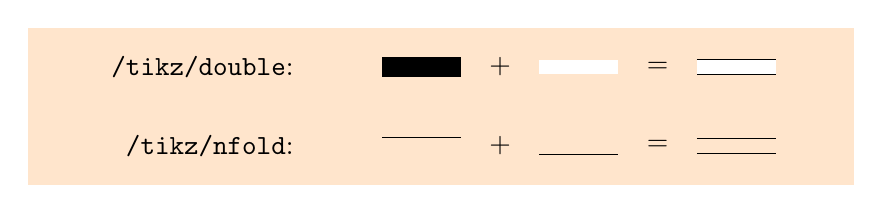
\begin{tikzpicture}[baseline=.5cm]
    \fill[orange!20] (-4.5,-.5) rectangle (6, 1.5);
    \node[left] at (-1,1) {\tikzdouble:};
    \draw[line width=7pt] (0,1) -- (1,1);
    \node at (1.5,1) {+};
    \draw[white, line width=5pt] (2,1) -- (3,1);
    \node at (3.5,1) {=};
    \draw[double distance=5pt] (4,1) -- (5,1);
    \node[left] at (-1,0) {\tikznfold:};
    \draw (0, 3pt) -- (1, 3pt);
    \node at (1.5,0) {+};
    \draw (2, -3pt) -- (3, -3pt);
    \node at (3.5,0) {=};
    \draw[double distance=5pt, nfold] (4,0) -- (5,0);
  \end{tikzpicture}
\end{equation}


\subsection{Issues with \tikzdouble}
\label{subsec:doubleIssues}
While the approach of \tikzdouble{} is very robust and efficient, it does have a few pitfalls:
\begin{itemize}
  \item Different types of visual glitches can occur in PDF renderers:
  \begin{itemize}
    \item One common issue is that the white foreground piece completely covers the black background piece at certain zoom levels, leading to the top or bottom part of the doubled path missing (depending on your PDF viewer and zoom level, this issue might be visible in \cref{eq:compareApproaches}).
    \item Another common glitch is the appearance of a thin horizontal line at the start and end of the doubled path (visible in most examples of curved paths if your viewer has this problem). The reason is that the larger black path in the background is not perfectly covered by the smaller white foreground piece, most likely due to rounding errors.
  \end{itemize}
  \item The approach assumes that the background has a uniform colour, and it is the user's responsibility to correctly set the background colour:
\begin{tkzexample}[latex=3.5cm]
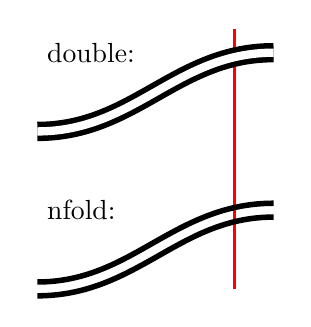
\begin{tikzpicture}
  \draw[red, line width=1pt] (2.5, 3.3) -- (2.5, 0);
  \draw[line width=2pt, double distance=3pt]
    (0,2) to[out=0, in=180] (3,3);
  \node[right] at (0,3) {double:};
  \draw[line width=2pt, double distance=3pt, nfold]
    (0,0) to[out=0, in=180] (3,1);
  \node[right] at (0,1) {nfold:};
\end{tikzpicture}
\end{tkzexample}
  \item Transparency does not work correctly:
\begin{tkzexample}[latex=3.5cm]
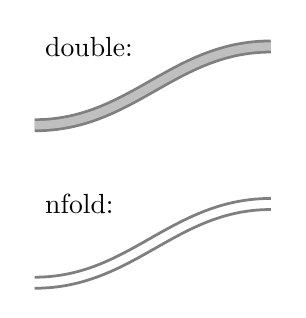
\begin{tikzpicture}[line width=1pt]
  \draw[double distance=3pt, opacity=.5]
    (0,2) to[out=0, in=180] (3,3);
  \draw[double distance=3pt, opacity=.5, nfold]
    (0,0) to[out=0, in=180] (3,1);
  \node[right] at (0,3) {double:};
  \node[right] at (0,1) {nfold:};
\end{tikzpicture}
\end{tkzexample}
  \item Triple and n-fold paths are not supported (although this could be implemented in principle).
\end{itemize}

\subsection{Issues with \tikznfold}

This package is far from perfect, and even if it were, there would still be some cases where the approach of \tikzdouble{} is better suited. Here are some shortcomings of \nfold:
\begin{itemize}
  \item \nfold{} struggles with high curvatures and wide paths: Let $\kappa(t)$ be the curvature of the path in a given point, and let $\texttt{double distance} = \alpha$. If $\kappa(t) > \frac{2}{\alpha}$ (i.e. the radius of the osculating circle is smaller than half the width of the path) for some $0 \leq t \leq 1$, the output of \nfold{} will not be correct:
\begin{tkzexample}[latex=3.5cm]
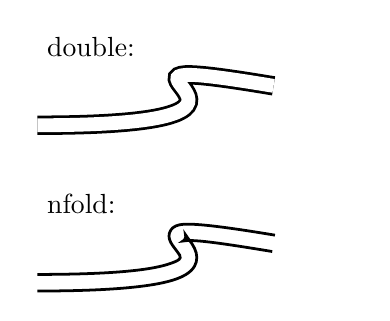
\begin{tikzpicture}
  \draw[double distance=5pt, line width=1pt]
    (0,2) .. controls (4,2) and (0,3) .. (3,2.5);
  \node[right] at (0,3) {double:};
  \draw[double distance=5pt, line width=1pt, nfold]
    (0,0) .. controls (4,0) and (0,1) .. (3,.5);
  \node[right] at (0,1) {nfold:};
\end{tikzpicture}
\end{tkzexample}
  Some, but not all of these cases raise warnings (this feature is on the wish list).
  \item Some rare cases of curves are not offset correctly. The reasons for that are discussed below in \cref{subsec:subdivisionUsed}. Usually, slightly changing the control points or values of the curve will fix the problem.
  \item Closing paths (i.e.\ using \texttt{-- cycle}) is not yet supported (this feature is on the wish list).
  \item \nfold{} is significantly slower than \tikzdouble. Part of the reason is that the construction is far more complex, other reasons can be fixed in principle. Specifically, the use of the \texttt{decorations} library is rather inefficient for this purpose.
  \item While I did my best trying to break \nfold{} with as many of TikZ' options as possible, there are most definitely some problematic options I have not tested. If you find any bugs, please report them at \todo{link}.
\end{itemize}


\section{Known issues}

\subsection{Fixable / wish list}

\begin{itemize}
  \item Closing paths (e.g.\ \texttt{-- cycle}) is not yet properly supported.
  \item The arrow detection is still quite rough and likely has some bugs. One known issue is that you cannot provide parameters to the arrow tips (e.g. \texttt{Implies[red]}).
  \item Similarly, redefining arrows does not have the desired effect (usually, it has no effect at all).
  \item It would not be very hard to check for too much curvature in the offsetting algorithm and throw warnings in these cases.
  \item Migrating away from the \texttt{decorations} library and integrating this algorithm more tightly with the rendering pipeline would be possible. I expect that doing so will significantly improve the performance and also fix most arrow-related issues. This idea is on the back burner for now, as it likely requires changes to the TikZ rendering pipeline. If the TikZ team shows interest in integrating this library, I will reconsider this.
  \item Discontinuous paths with an arrow tip at the start are rendered differently in \tikzdouble{} and \nfold. As I do not really see a use case for such paths (and a rendering pipeline integration would likely fix it anyway), this issue is not a priority for now.
\end{itemize}

\subsection{Impossible or very hard to fix}
\begin{itemize}
  \item Correctly rendering paths with too much curvature is borderline impossible with this approach. This is one of the cases where using \tikzdouble{} is the only viable option.
  \item Curves of \nfold{} slightly deviate from the curves of \tikzdouble{} near joins with a non-zero angle:
\begin{tkzexample}[latex=3.5cm]
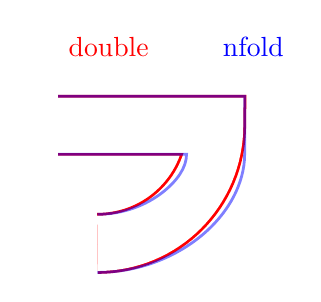
\begin{tikzpicture}[line width=1pt]
  \draw[red, double distance=20pt]
    (0,2) -- (2,2) to [out=-90, in=0] (.5,.5);
  \draw[blue, double distance=20pt, opacity=.5, nfold]
    (0,2) -- (2,2) to [out=-90, in=0] (.5,.5);
  \node[right, red] at (0,3) {double};
  \node[left, blue] at (3, 3) {nfold};
\end{tikzpicture}
\end{tkzexample}
  This cannot be fixed without extensive use of the \texttt{intersections} library, hurting the performance, and the result might still not look great for orders $\geq 3$.
  \item changing joins in \verb|\pgfsys@beginscope| without an accompanying \TeX{} group may cause inconsistent behaviour in the joins. For example,
\begin{tkzexample}[latex=2cm]
\makeatletter
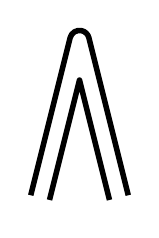
\begin{tikzpicture}[line join=miter, line width=2pt]
  \pgfsys@beginscope
    \pgfsetroundjoin
  \pgfsys@endscope
  \draw[double distance=5pt, nfold] (0,0) -- (.5,2) -- (1,0);
\end{tikzpicture}
\makeatother
\end{tkzexample}
  has \texttt{round} joins on the large path, but \texttt{miter} joins on the constituent paths. This problem does not occur with \verb|\pgfscope|.
\end{itemize}

\section{The basic layer \texttt{pgf} commands}

This package also provides some basic layer commands for offsetting curves and straight lines. Use
\begin{verbatim}
\usepgflibrary{bezieroffset}
\end{verbatim}
to only import the base layer library. The following commands are provided:
\begin{itemize}
  \item \verb|\pgfoffsetcurve|: This macro draws the parallel of a Bézier curve. It takes five parameters, the first four being the four control points of the Bézier curve (e.g.\ in the form of \verb|\pgfpoint{}{}|), the fifth parameter is the distance by which the curve should be offset. A negative value offsets the curve in the opposite direction. This macro begins with a \verb|\pgfpointmoveto| to the offset first control point.
  \item \verb|\pgfoffsetcurvenomove|: The only difference to the previous macro is that this version does not move to the offset first control point. This is useful if one wants to offset an uninterrupted path consisting of several curves. The output will only be correct if the previous path segment ends on the offset first control point.
  \item \verb|\pgfoffsetline|: This macro offsets a straight line. It takes two points and the distance as parameters.
  \item \verb|\pgfoffsetlinenomove|: This macro is analogous to \verb|\pgfoffsetcurvenomove|.
\end{itemize}


\appendix
\newpage
\section{The offsetting algorithm}

This algorithm is based on an algorithm by \href{https://github.com/Pomax/}{Pomax}. See \href{https://pomax.github.io/bezierinfo/#offsetting}{A Primer on Bézier curves}, the source code can be found \href{https://github.com/Pomax/bezierinfo/blob/bcfce2149fa5e5540a2a2605986adab3b2a9a3bf/js/graphics-element/lib/bezierjs/bezier.js}{here}.

\subsection{Simple and fully simple Bézier curves}

Throughout this section the term ``Bézier curve'' refers to a cubic Bézier curve, which is defined by four points $(A_1, A_2, A_3, A_4)$.

As explained in the aforementioned source, in almost all cases the parallel of a Bézier curve is not exactly a Bézier curve itself. To approximate the parallel using Bézier curves, we therefore first divide the given curve into ``simple'' segments which can be offset with reasonable accuracy. The following defines a simple segment:
\begin{definition}
  \label{def:simpleCurve}
  A Bézier curve $(A_1, A_2, A_3, A_4)$ is \emph{simple} if
  \begin{enumerate}
    \item the points $A_2$ and $A_3$ lie on the same side of the line $\overline{A_1A_4}$,
    \item the absolute angle between the tangents in $A_1$ and $A_4$ is at most $\pi/3$ (i.e.\ the cosine is no smaller than $0.5$), and
    \item the distances fulfil $\overline{A_1A_2} + \overline{A_3A_4} \leq \overline{A_1A_4}$.\footnote{The reference only uses the first two conditions.}
  \end{enumerate}
\end{definition}
\begin{definition}
  \label{def:fullySimpleCurve}
  A Bézier curve $(A_1, A_2, A_3, A_4)$ is \emph{fully simple}\footnote{This terminology is not used in the source.} if all of its segments are simple in the sense of \cref{def:simpleCurve}.
\end{definition}
In order to offset an arbitrary Bézier curve we split it into fully simple segments.

\subsection{Subdivision}

It is well known that at every point $0 < t < 1$, a Bézier curve $A = (A_1, A_2, A_3, A_4)$ can be subdivided into two Bézier curves $B$ and $C$ using de Casteljau's algorithm (which naturally fulfil $A_1 = B_1$ and $A_4 = C_4$). A more or less heuristic fact is that $B$ and $C$ are ``more likely'' to be simple than $A$ (if you can prove any of the statements here, please contact me). Hence, if one wants to offset a non-simple curve $A$, one could try to subdivide $A$ until all of its segments are simple, then offset each segment.

\subsection{Pomax' approach}
The original approach by Pomax consists of two passes. The first pass subdivides $A$ on all extrema in $x$ or $y$. In a second pass, each segment $A^{(i)}$ is made simple in steps of $t \mapsto t + 0.01$, roughly using the following pseudocode:
\begin{samepage}
\begin{verbatim}
  t_1 = t_2 = 0.0
  while t_2 < 1.0:
    S = segment(A from t_1 to t_2+0.01)
    if not isSimple(S):
      segments += [S]
      t_1 = t_2
    t_2 += 0.01
\end{verbatim}
\end{samepage}
Essentially, this verifies with great certainty that the segment is fully simple in the sense of 

The main reason this approach is not used in this library is performance, as the library is slow enough already. Other minor reasons include that the original approach is not invariant under reversals or rotations: Reversing and/or rotating a curve yields a different subdivision and hence potentially a slightly different-looking curve.

\subsection{The approach used here}
\label{subsec:subdivisionUsed}
In this library, we instead take a recursive approach:
\begin{verbatim}
  def split(A, level):
    if isSimple(A):
      segments += [A]
    else:
      if level < 0:
        Display a warning
        segments += [A]
      else:
        first, second = split(A, t=0.5)
        split(first, level-1)
        split(second, level-1)
\end{verbatim}
The default maximum depth is 5, so the curve is split into at most $2^5 = 32$ segments. This has the downside that some simple but not fully simple curves may remain undetected and be offset slightly incorrectly. If you encounter examples of such curves with bad outputs or if you have any ideas for additional constraints to add to \cref{def:simpleCurve} that can be checked with reasonable computational effort, please be in touch.


\subsection{Offsetting simple Bézier curves}

Disregarding edge cases (which will be discussed later), offsetting the curve works as follows:
\begin{enumerate}
  \item Construct lines orthogonal to the tangent in $A_1$ and $A_4$ and find their intersection. This point is called the \emph{origin} of the curve.
  \item The new control points $A'_1$ and $A'_4$ are given by $A_1$ and $A_4$ offset orthogonally to the tangent.
  \item Construct a ray from $A'_1$ parallel to the tangent in $A_1$, and construct another ray from the origin through $A_2$. Now $A'_2$ is given by the intersection of those rays.
  \item $A'_3$ can be constructed similarly.
\end{enumerate}
The construction is shown in the following picture:
\[
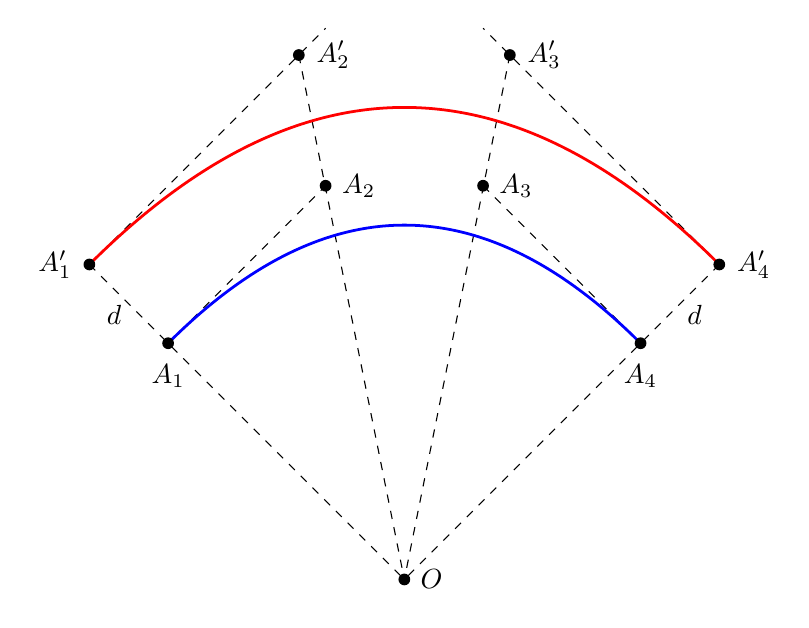
\begin{tikzpicture}[every node/.append style={inner sep=1.5pt, circle, fill}]
  \coordinate (A1) at (-3, 0);
  \coordinate (A2) at (-1, 2);
  \coordinate (A3) at (1, 2);
  \coordinate (A4) at (3, 0);
  \coordinate (A1p) at (-4, 1);
  \coordinate (A4p) at (4, 1);
  \coordinate (A2p) at ($(A1p) + 1.33*(2,2)$);
  \coordinate (A3p) at ($(A4p) + 1.33*(-2,2)$);
  \coordinate (O) at (0, -3);
  \draw[dashed] (A1) -- (A2) (A3) -- (A4);
  \draw[dashed] (A1p) -- +(3,3) (A4p) -- +(-3,3);
  \draw[dashed] (A1p) -- (O) node[pos=.12, below left, fill=none] {$d$} (A4p) -- (O) node[pos=.12, below right, fill=none] {$d$};
  \draw[dashed] (A2p) -- (O) (A3p) -- (O);
  \draw[line width=1pt, blue] (A1) .. controls (A2) and (A3) .. (A4);
  \draw[line width=1pt, red] (A1p) .. controls (A2p) and (A3p) .. (A4p);
  \node[label={below:$A_1$}] at (A1) {};
  \node[label={right:$A_2$}] at (A2) {};
  \node[label={right:$A_3$}] at (A3) {};
  \node[label={below:$A_4$}] at (A4) {};
  \node[label={left:$A'_1$}] at (A1p) {};
  \node[label={right:$A'_2$}] at (A2p) {};
  \node[label={right:$A'_3$}] at (A3p) {};
  \node[label={right:$A'_4$}] at (A4p) {};
  \node[label={right:$O$}] at (O) {};
\end{tikzpicture}
\]

\subsection{Removing singularities}

Clearly, as the angle between $\overrightarrow{A_1A_2}$ and $\overrightarrow{A_3A_4}$ decreases, the origin approaches infinity. Computing the control points $(A'_i)$ by computing the coordinates of $O$ is therefore not numerically stable for almost straight curves. However, we can get around this problem using elementary geometry. Constructing $A'_1$ and $A'_4$ is independent of the location of the origin, so the only difficult part is computing the distances $\overline{A'_1A'_2}$ and $\overline{A'_3A'_4}$. We find
\begin{equation}
  \frac{\overline{A'_1A'_2}}{\overline{A_1A_2}} = \frac{\overline{OA'_1}}{\overline{OA_1}} = 1 + \frac{d}{\overline{OA_1}} \implies \overline{A'_1A'_2} = \overline{A_1A_2} \left(1 + d \cdot \frac{1}{\overline{OA_1}}\right)
\end{equation}
which is regular as $O$ approaches infinity. Now we to determine the inverse of $\overline{OA_1}$, which can be computed using the law of sines:
\[
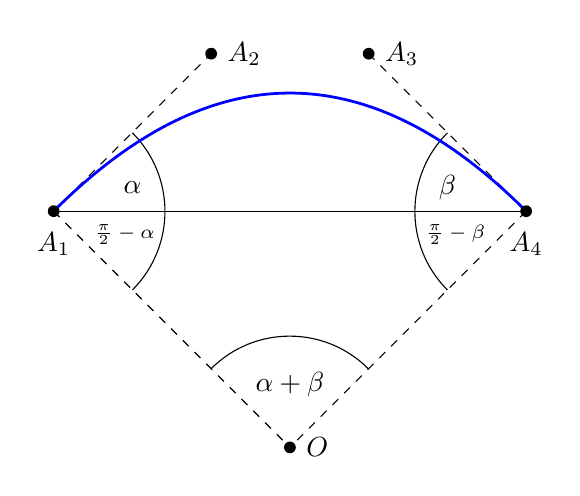
\begin{tikzpicture}[every node/.append style={inner sep=1.5pt, circle, fill}]
  \coordinate (A1) at (-3, 0);
  \coordinate (A2) at (-1, 2);
  \coordinate (A3) at (1, 2);
  \coordinate (A4) at (3, 0);
  \coordinate (O) at (0, -3);
  \draw[dashed] (A1) -- (A2) (A3) -- (A4);
  \draw[dashed] (A1) -- (O) (A4) -- (O);
  \draw (A1) -- (A4);
  \draw (-2,-1) arc[start angle=-45, end angle=45, radius=1.41cm];
  \draw ( 2,-1) arc[start angle=180+45, end angle=180-45, radius=1.41cm];
  \draw (-1,-2) arc[start angle=180-45, end angle=45, radius=1.41cm];
  \draw[line width=1pt, blue] (A1) .. controls (A2) and (A3) .. (A4);
  \node[label={below:$A_1$}] at (A1) {};
  \node[label={right:$A_2$}] at (A2) {};
  \node[label={right:$A_3$}] at (A3) {};
  \node[label={below:$A_4$}] at (A4) {};
  \node[fill=none] at (-2,.3) {$\alpha$};
  \node[fill=none] at (-2.1,-.3) {\scriptsize$\frac{\pi}{2}-\alpha$};
  \node[fill=none] at ( 2,.3) {$\beta$};
  \node[fill=none] at ( 2.1,-.3) {\scriptsize$\frac{\pi}{2}-\beta$};
  \node[fill=none] at (0,-2.2) {$\alpha+\beta$};
  \node[label={right:$O$}] at (O) {};
\end{tikzpicture}
\]
\begin{equation}
  \frac{\sin(\tfrac{\pi}{2} - \alpha)}{\overline{OA_4}} = \frac{\sin(\alpha + \beta)}{\overline{A_1A_4}} = \frac{\sin(\tfrac{\pi}{2} - \beta)}{\overline{OA_1}} \implies \frac{1}{\overline{OA_1}} =  \frac{1}{\overline{A_1A_4}}\cdot\frac{\sin(\alpha + \beta)}{\cos(\beta)} \ .
\end{equation}
Note that $-\tfrac{\pi}{2} < \beta < \tfrac{\pi}{2}$ (and hence $\cos(\beta) > 0$) is guaranteed if the curve is simple --- in fact, simplicity guarantees $\alpha \cdot \beta > 0$ and $|\alpha| + |\beta| \leq \tfrac{\pi}{3}$. Using the sine addition theorem we can further rewrite the fraction to
\begin{equation}
  \frac{\sin(\alpha + \beta)}{\cos(\beta)} = \sin(\alpha) + \cos(\alpha) \frac{\sin(\beta)}{\cos(\beta)} \ ,
\end{equation}
and all of these terms can be computed directly from dot and cross products of vectors between the original control points. To summarise, let $\vv_{ij} := \overrightarrow{A_iA_j}$, and let $\vv_0$, $\vv_1$ be the normalised tangents at $t=0$ and $t=1$, respectively (see \cref{subsec:stabilisation} how they are computed). Then
\begin{equation}
% for checking
  \overline{A'_1A'_2} = \overline{A_1A_2} + \frac{d}{\overline{A_1A_4}^2}\cdot\left(\vv_{12} \times \vv_{14} - \vv_{12}\cdot\vv_{14} \frac{\vv_{14}\times\tv_1}{\vv_{14}\cdot\tv_1} \right) \ .
\end{equation}
Let furthermore $\uv_{ij} := \vv_{ij}/|\vv_{ij}|$ be the normalised vectors. Then we find
\begin{equation}%
  \label{eq:finalPrimeDistance}
  \begin{aligned}
    \overline{A'_1A'_2} &= \overline{A_1A_2} + \frac{d}{\overline{A_1A_4}} \left(\vv_{12} \times \uv_{14} - \vv_{12}\cdot\uv_{14} \frac{\uv_{14}\times\tv_1}{\uv_{14}\cdot\tv_1} \right) \ , \\
    \overline{A'_4A'_3} &= \overline{A_4A_3} + \frac{d}{\overline{A_1A_4}} \left(\vv_{43} \times \uv_{14} - \vv_{43}\cdot\uv_{14} \frac{\uv_{14}\times\tv_0}{\uv_{14}\cdot\tv_0} \right) \ .
  \end{aligned}
\end{equation}



\subsection{Edge cases}

\subsubsection{Overlaps: $A_i = A_{i+1}$}

If there is one overlap $A_1=A_2$, $A_2=A_3$ or $A_3=A_4$, the cubic Bézier curve reduces to a quadratic one. For two overlaps, we get a linear Bézier curve (i.e.\ a straight line), and for three overlaps we get a point. The main problem to watch out for is that the tangents $\tv_0$ and $\tv_1$ need to be computed differently:
\begin{itemize}
  \item If $A_1 \neq A_2$, we find $\tv_0 = \uv_{12}$.
  \item If $A_1 = A_2 \neq A_3$, we find $\tv_0 = \uv_{13}$.\footnote{This implicitly assumes a regular reparametrisation of the curve (e.g. a parametrisation over arc length); the usual parametrisation has a gradient of zero at $t=0$.}
  \item If $A_1 = A_2 = A_3 \neq A_4$, we find $\tv_0 = \uv_{14}$.
  \item If $A_1 = A_2 = A_3 = A_4$, the curve is just a point and the tangent is not defined. The implementation defaults to $\tv_0 = (1,0)$.
\end{itemize}
The analogous statement hold for $\tv_1$. In practice we test for approximate, not exact equality.

\subsubsection{Overlaps $A_1 = A_4$}

\Cref{eq:finalPrimeDistance} has one remaining singularity, namely for $A_1 \approx A_4$. This singularity is fundamental and not an artefact: As $A_1$ approaches $A_4$ while $\overline{A_1A_2}$ and $\overline{A_3A_4}$ stay constant, $O$ also approaches $A_4$, hence the angle between $\overrightarrow{A_1A_2}$ and $\overrightarrow{OA_2}$ approaches zero, sending the intersection point $A'_2$ to infinity.

A closer inspection of this special case reveals a number of sub-cases:
\begin{itemize}
  \item Fully degenerate curves with $A_1 \approx A_2 \approx A_3 \approx A_4$. Offsetting these curves in a stable manner is impossible, as the gradient and hence the direction in which to offset is numerically unstable. Rendering such curves will hardly have any output at all anyway. See below in \cref{subsec:stabilisation} how this case is handled.
  \item Non-trivial loops with $\overline{A_1A_2} \gg \overline{A_1A_4}$ and/or $\overline{A_3A_4} \gg \overline{A_1A_4}$, $|\alpha| + |\beta| \geq \tfrac{\pi}{3}$. Such curves violate the second and third condition of \cref{def:simpleCurve}, for example:
  \[
  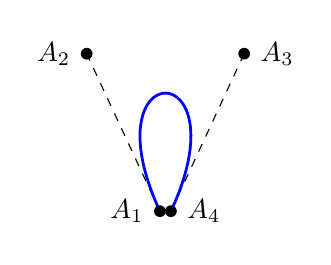
\begin{tikzpicture}[every node/.append style={inner sep=1.5pt, circle, fill}]
    \coordinate (A1) at (-.07, 0);
    \coordinate (A2) at (-1, 2);
    \coordinate (A3) at (1, 2);
    \coordinate (A4) at (.07, 0);
    \draw[dashed] (A1) -- (A2) (A3) -- (A4);
    \draw[line width=1pt, blue] (A1) .. controls (A2) and (A3) .. (A4);
    \node[label={left:$A_1$}] at (A1) {};
    \node[label={left:$A_2$}] at (A2) {};
    \node[label={right:$A_3$}] at (A3) {};
    \node[label={right:$A_4$}] at (A4) {};
  \end{tikzpicture}
  \]
  \item Curves with $\overline{A_1A_2} \gg \overline{A_1A_4}$ and/or $\overline{A_3A_4} \gg \overline{A_1A_4}$,  $|\alpha| + |\beta| < \tfrac{\pi}{3}$: Such curves violate the third condition of \cref{def:simpleCurve}, for example:
  \[
  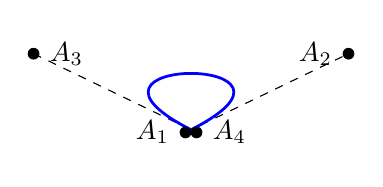
\begin{tikzpicture}[every node/.append style={inner sep=1.5pt, circle, fill}]
    \coordinate (A1) at (-.07, 0);
    \coordinate (A3) at (-2, 1);
    \coordinate (A2) at (2, 1);
    \coordinate (A4) at (.07, 0);
    \draw[dashed] (A1) -- (A2) (A3) -- (A4);
    \draw[line width=1pt, blue] (A1) .. controls (A2) and (A3) .. (A4);
    \node[label={left:$A_1$}] at (A1) {};
    \node[label={left:$A_2$}] at (A2) {};
    \node[label={right:$A_3$}] at (A3) {};
    \node[label={right:$A_4$}] at (A4) {};
  \end{tikzpicture}
  \]
\end{itemize}

\subsection{Stabilising the offsetting algorithm for non-simple curves}
\label{subsec:stabilisation}

As seen in \cref{subsec:subdivisionUsed}, there are cases where the offsetting algorithm will be called on non-simple curves. In such cases it is essential that the code does not crash (e.g. from division by zero), and that the output produced is at least somewhat sensible. The following measures are taken:
\begin{itemize}
  \item If $\overline{A_1A_4}$ is very close to zero,\footnote{Clamping the fraction $d/\overline{A_1A_4}$ to some maximum value did not work well, as it had a tendency of producing false positives.} we set $\overline{A'_1A'_2} = \overline{A_1A_2}$ and $\overline{A'_3A'_4} = \overline{A_3A_4}$, forming a rather rough approximation of the parallel curve. This causes a warning to be logged.
  \item For simple curves we find $\uv_{14}\cdot\uv_{34} \geq 0.5$ in the denominator. Therefore, for non-simple curves, the denominator is clamped to $[0.5, 1.0]$, preventing division by zero.
\end{itemize}


\end{document}
